\documentclass[letterpaper,10pt]{article}

\usepackage{titling}
\usepackage{listings}
\usepackage{url}
\usepackage{setspace}
\usepackage{subfig}
\usepackage{sectsty}
\usepackage{pdfpages}
\usepackage{colortbl}
\usepackage{multirow}
\usepackage{relsize}
\usepackage{amsmath}
\usepackage{fancyvrb}
\usepackage{amsmath,amssymb,amsthm,graphicx,xspace}
\usepackage[titlenotnumbered,noend,noline]{algorithm2e}
\usepackage[compact]{titlesec}
\usepackage{paratype} 
\usepackage[T1]{fontenc}
\usepackage{tikz}
\usetikzlibrary{arrows,automata,shapes,trees,matrix,chains,scopes,positioning,calc}
\tikzstyle{block} = [rectangle, draw, fill=blue!20, 
    text width=2.5em, text centered, rounded corners, minimum height=2em]
\tikzstyle{bw} = [rectangle, draw, fill=blue!20, 
    text width=4em, text centered, rounded corners, minimum height=2em]

\definecolor{namerow}{cmyk}{.40,.40,.40,.40}
\definecolor{namecol}{cmyk}{.40,.40,.40,.40}

\let\LaTeXtitle\title
\renewcommand{\title}[1]{\LaTeXtitle{\textsf{#1}}}


\newcommand{\handout}[5]{
  \noindent
  \begin{center}
  \framebox{
    \vbox{
      \hbox to 5.78in { {\bf ECE254: Operating Systems and Systems Programming } \hfill #2 }
      \vspace{4mm}
      \hbox to 5.78in { {\Large \hfill #4  \hfill} }
      \vspace{2mm}
      \hbox to 5.78in { {\em #3 \hfill} }
    }
  }
  \end{center}
  \vspace*{4mm}
}

\newcommand{\lecture}[3]{\handout{#1}{#2}{#3}{Lecture #1}}
\newcommand{\tuple}[1]{\ensuremath{\left\langle #1 \right\rangle}\xspace}

\addtolength{\oddsidemargin}{-1.000in}
\addtolength{\evensidemargin}{-0.500in}
\addtolength{\textwidth}{2.0in}
\addtolength{\topmargin}{-1.000in}
\addtolength{\textheight}{1.75in}
\addtolength{\parskip}{\baselineskip}
\setlength{\parindent}{0in}
\renewcommand{\baselinestretch}{1.5}
\newcommand{\term}{Spring 2015}

\singlespace


\begin{document}

\lecture{ 8 --- Threads }{\term}{Jeff Zarnett}

\section*{Threads}

Recall our earlier examination of the process. A process has three major components: an executable program, the data created/needed by the program, and the execution context of the program (files opened, resources allocated, et cetera). A process has at least one \textit{thread}, and can have many.

The term ``thread'' is a short form of \textit{Thread of Execution}. A thread of execution is a sequence of executable commands that can be scheduled to run on the CPU. Threads also have some state (where in the sequence of executable commands the program is) and stores some local variables. Most programs you will write in other courses had only one thread; that is, your program's code is executed one statement at a time.

A multithreaded program is one that uses more than one thread, at least some of the time. When a program is started, it begins with an initial thread (where the \texttt{main} method is) and that main thread can create some additional threads if needed. Note that threads can be created and destroyed within a program dynamically: a thread can be created to handle a specific background task, like writing changes to the database, and will terminate when it is done. Or a created thread might be persistent.

See the figure below, which illustrates some possible organizations for processes and threads in different programs:

\begin{center}
	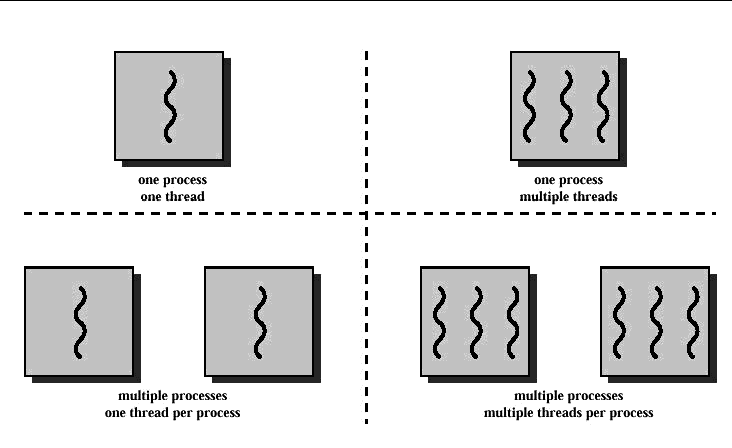
\includegraphics[width=0.625\textwidth]{images/mthread.png}\\
	Possible organizations of processes and threads~\cite{mthread}.
\end{center}

In a process that has multiple threads, each thread has its own~\cite{osi}:
\begin{enumerate}
	\item Thread execution state (like process state: running, ready, blocked...).
	\item Saved thread context when not running.
	\item Execution stack.
	\item Local variables.
	\item Access to the memory and resources of the process (shared with all threads in that process).
\end{enumerate}

Or, to represent this visually:

\begin{center}
	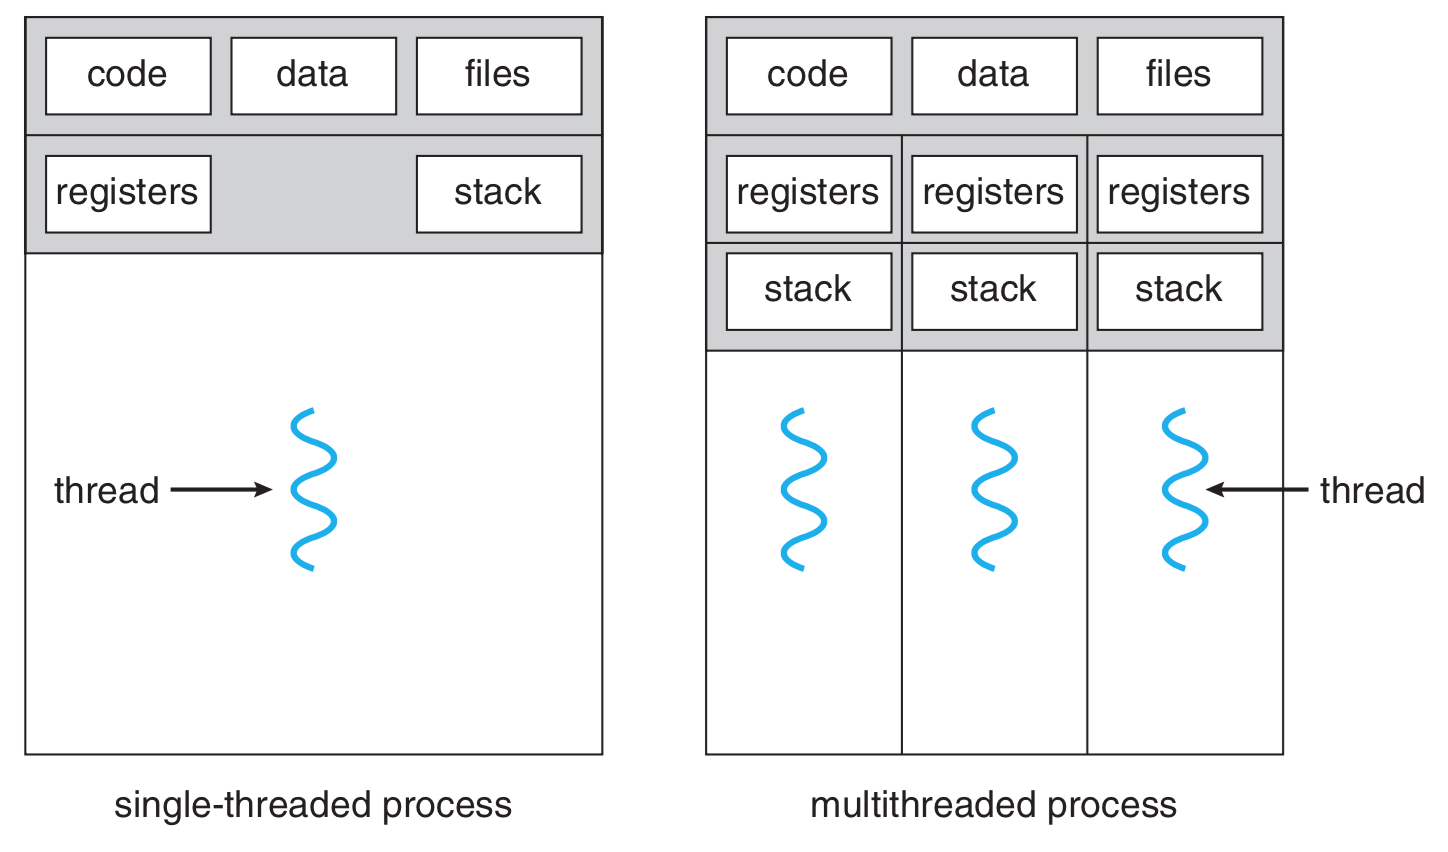
\includegraphics[width=0.625\textwidth]{images/mthread2.png}\\
	A single threaded and a multithreaded process compared side-by-side~\cite{osc}.
\end{center}

All the threads of a process share the state and resources of the process. If one thread opens a file, other threads in that process can also access that file.

The way programs are written now, there are few if any that are not in some way multithreaded. One common way of dividing up the program into threads is to separate the user interface from a time-consuming action. 

Consider a file-transfer program. If the user interface and upload method share a thread, once a file upload has started, the user will not be able to use the UI anymore (and Windows will put the dreaded ``(Not Responding)'' at the end of its dialog title), even to click the button that cancels the upload. For some reason, users hate that. 

We have two options for how to alleviate this problem: when an upload is ready to start, we can call \texttt{fork} and create a new process to do the upload, or we can spawn  new thread. In either case, the newly created entity will handle the upload of the file. The UI remains responsive, because the UI thread is not waiting for the upload method to complete.

\subsection*{Motivation for Threads}

Why choose threads rather than creating a new process? The primary, but not sole, motivation is performance:
\begin{enumerate}
	\item Creating a new thread is much faster than creating a new process. In fact, thread creation is on the order of ten times faster~\cite{machThreads}.
	\item Terminating and cleaning up a thread is faster than terminating and cleaning up a process.
	\item It takes less time to switch between two threads within the same process (because less data needs to be stored/restored). In Solaris, for example, switching between processes is about five times slower than switching between threads~\cite{osc}.
	\item Because threads share the same memory space, for two threads to communicate, they do not have to use any of the IPC mechanisms; they can just communicate directly.
	\item As in the file transfer program, use of threads allows the program to be responsive even when a part of the program is blocked.
\end{enumerate}

This last advantages, background work, is one of four common examples of the uses of threads in a general purpose operating system~\cite{insideOS2}:
\begin{enumerate}
	\item \textbf{Foreground and Background Work:} as already examined, the ability to run something in the background to keep the program responsive.
	\item \textbf{Asynchronous processing}: for example, to protect against power failure or a crash, a word processor may write the document data in main memory to disk periodically. This can be done as a background task so it does not disrupt the user's workflow.
	\item \textbf{Speed of Execution:} a multithreaded program can get more done in the same amount of time. Just as the OS can run a different program when the executing program gets blocked (say, on a disk read), if one thread is blocked, another thread may execute.
	\item \textbf{Modular Structure:} a program that does several different things may be given structure through threads.
\end{enumerate}

There are some drawbacks, however: there is no protection between threads in the same process: so one thread can easily mess with the memory being used by another thread. This once again brings us to the subject of co-ordination, which will follow the discussion of threads.

Also, if any thread encounters an error (such as a division by zero or Segmentation Fault), the whole process might be terminated by the operating system. If the program has multiple processes for different parts, then the other processes will not be affected; if the program has multiple threads and they all share the same process, then any thread encountering an error might bring all of them to a halt.


\subsection*{Thread States}
Each individual thread will have its own state. We said earlier that a process may have seven states, but the model for thread state will be the somewhat simpler five-state model. If a process is swapped out of memory, all its threads will be swapped out; when that process is swapped in to memory, all the threads will be swapped in. Therefore we do not need to consider whether a thread is in memory or swapped; hence the five-state model, reproduced once again below:

\begin{center}
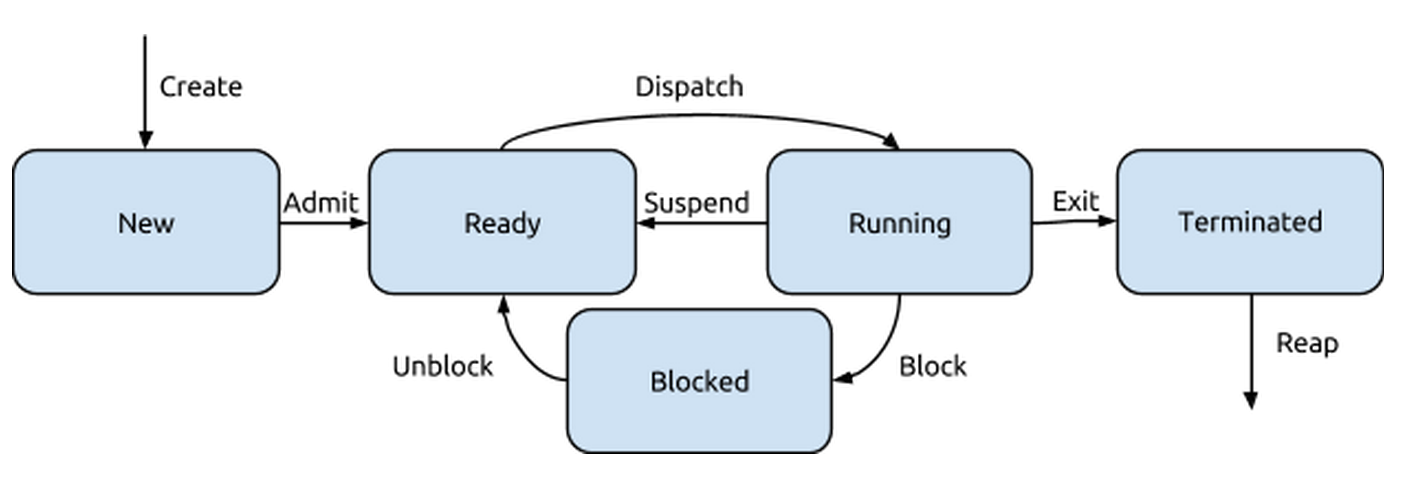
\includegraphics[width=0.85\textwidth]{images/5-state-model.png}\\
State diagram for the five-state model.
\end{center}

The transitions work the same way as the state transitions for a process. As with a process, a thread in any state can transition to terminated even though that is not shown on the diagram. When a process is terminated, all its threads are terminated, regardless of what state it is in. The example we started with, the file transfer upload being cancelled, is an example of termination we should consider: thread cancellation.

\subsection*{Thread Cancellation}
Thread cancellation is exactly what it sounds like: a running thread will be terminated before it has finished its work. Once the user presses the cancel button on the file upload, we want to stop the upload task that was in progress. The thread that we are going to cancel is called the \textit{target} (because we shoot targets, I guess) and there are two ways a thread might get cancelled~\cite{osc}:

\begin{enumerate}
	\item \textbf{Asynchronous Cancellation:} One thread immediately terminates the target.
	\item \textbf{Deferred Cancellation:} The target is informed that it is cancelled; the target is responsible for checking regularly if it is terminated, allowing it to clean itself up properly. 
\end{enumerate}

For example, in Android, a background task has a function \texttt{isCancelled} that returns a boolean value. If we cancel a task then the \texttt{isCancelled} value returns true, but on its own that does not actually impact the task directly. The task itself is responsible for checking if \texttt{isCancelled} is true and stopping its activity and cleaning up (closing open files, etc.) before it terminates. This is deferred cancellation, and it's possible, though generally poor programming practice, to never check for cancellation.

Given that a thread can effectively ignore a cancellation if it is the deferred cancellation type, why would we ever choose that over asynchronous cancellation? Suppose the thread we are cancelling has some resources. If the thread is terminated in a disorderly fashion, the operating system may not reclaim all resources from that thread. Thus a resource may appear to be in use even though it is not, denying that resource to other threads and processes that may want to use it~\cite{osc}.

\subsection*{Thread Types}

There are two categories of threads in implementation: \textit{user-level} threads (ULTs) and \textit{kernel-level} threads (KLTs -- sometimes also called a lightweight process). ULTs run at the user level and KLTs run at the kernel level.

There are three possible approaches: (1) all threads are user level; (2) all threads are kernel level; and (3) a combination of both approaches. See the diagram below:

\begin{center}
	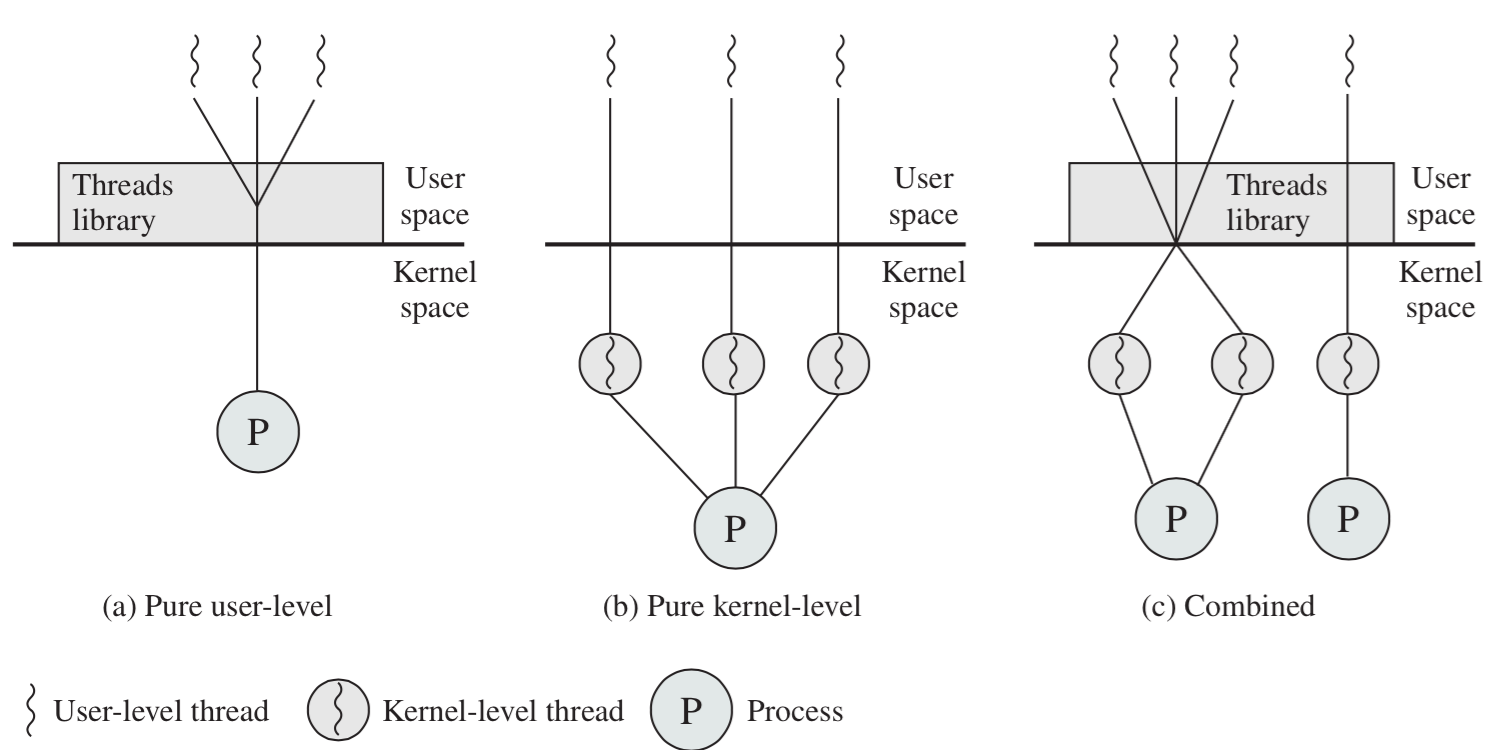
\includegraphics[width=0.85\textwidth]{images/thread-types.png}\\
	User and Kernel-Level Threads~\cite{osi}.
\end{center}


If the operating system in question does not support threads, we can still have multithreaded programming through user level threads in some sort of threads library. The library handles creation, management, and cleanup of threads. The kernel is unaware of the existence of the user level threads and it is therefore the responsibility of the threads library or the application to manage the threads. 

There are three advantages to using user-level threads~\cite{osi}:
\begin{enumerate}
	\item Thread switches do not require kernel mode privileges, because the thread library is in the user-side. Thus we do not have to switch to kernel mode and back for each thread switch.
	\item Scheduling can be something the program decides rather than leaving it to operating system policy. 
	\item Portability: the program can run in a multithreaded way even if the kernel does not support multiple threads.
\end{enumerate}

As far as the kernel is concerned, there is only one thread for that process. Thus, if any of the threads in the process block (such as making an I/O request), the whole process will be blocked. But there is a solution to this called \textit{jacketing}: conversion of a blocking system call into a non-blocking system call. Instead of calling the system call directly, the program calls the thread library's version of the system call. The jacket routine checks if the request will result in the application being blocked and can decide instead to consider the requesting thread blocked and switch to another one, preventing the OS from blocking the whole process.

The kernel level threads approach is taken by Windows, for example. The kernel is responsible for all thread management and it overcomes one of the weaknesses of the ULT approach: if one thread in a process is blocked, the others may continue. Another positive feature is that the kernel routines themselves may be multithreaded~\cite{osi}.

The disadvantage of this is the opposite of the advantage of the ULT: a thread switch involves entering kernel mode with a \texttt{trap} and then returning from kernel mode to user mode (which does, of course, take time).

We can, certainly, combine both approaches where user level and kernel level threads co-exist in the system. This is common as any system that has kernel level threads can still run applications that use a thread library. 

To look at this from another angle, we can consider the relationships between user and kernel level threads, of which we will consider three: Many-To-One, One-To-One, and Many-To-Many.

\paragraph{The Many-To-One Model.} In this model, many user level threads are mapped to one kernel thread. Thread management is done in the user space; this is what we see with ULTs only. Few modern operating systems take this approach; most everything these days has at least some support for KLTs.

\paragraph{The One-To-One Model.} This is what happens when we have KLTs only. Creating a new user level thread results immediately in creating a kernel level thread to correspond to it. Linux and Windows, notably, follow this approach, with some limitations on the number of threads that can be created in the system~\cite{osc}.

\paragraph{The Many-To-Many Model.} This maps many ULTs to a smaller or equal number of kernel threads. This approach provides maximal concurrency in executing a single program.

You will note there is no One-To-Many model. This is because it makes no sense for one user thread to be mapped to multiple kernel threads. After all, a user thread needs a kernel thread only some of the time and having multiple kernel threads waiting around to serve the user level thread is wasteful.

All three approaches are shown in the diagram below:

\begin{center}
	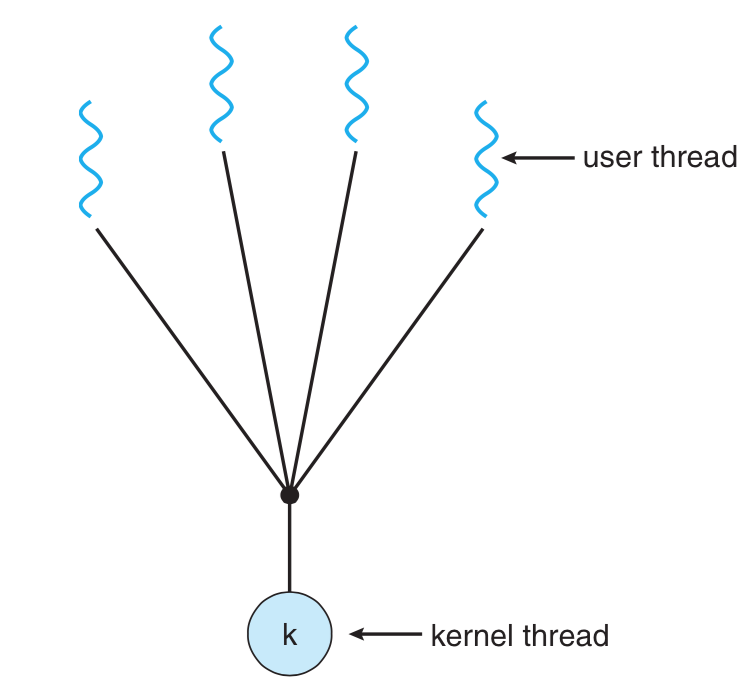
\includegraphics[width=0.32\textwidth]{images/threads-manytoone.png}
	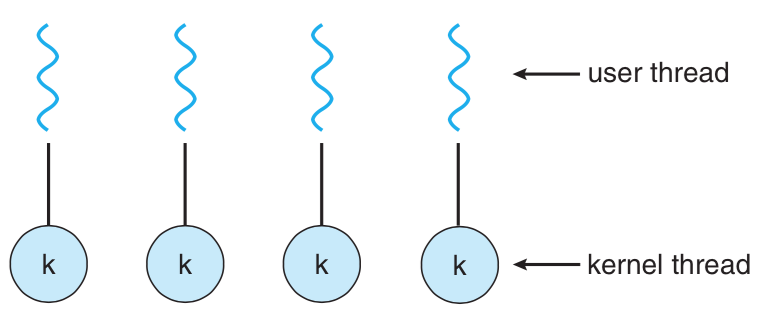
\includegraphics[width=0.32\textwidth]{images/threads-onetoone.png}
	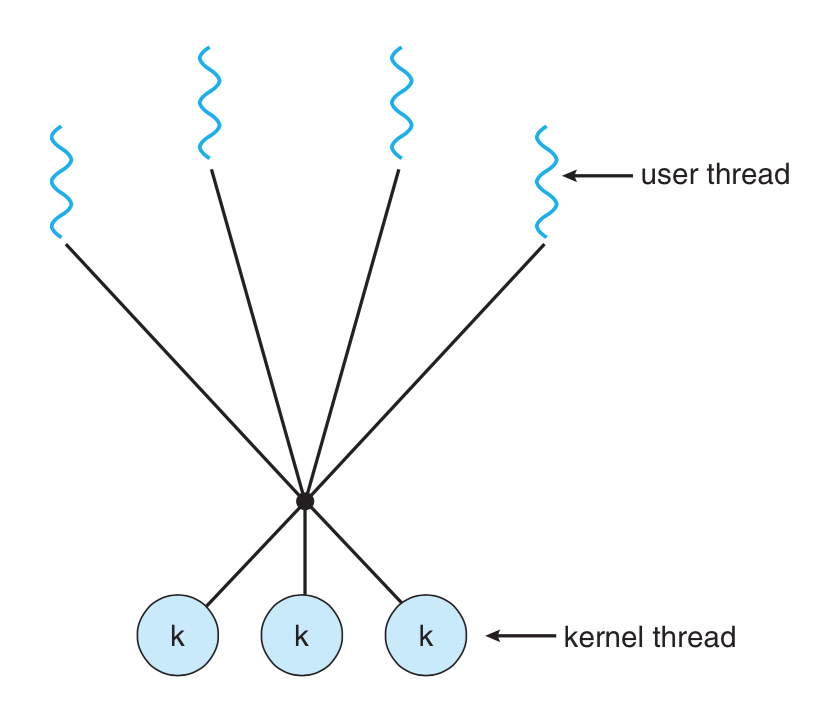
\includegraphics[width=0.32\textwidth]{images/threads-manytomany.png}\\
	Left to right: User to Kernel level thread mappings: Many-To-One, One-To-One, and Many-To-Many~\cite{osc}.
\end{center}

\bibliographystyle{alpha}
\bibliography{254}


\end{document}